\documentclass{article}

\usepackage[utf8]{inputenc}
\usepackage{hyperref}
\usepackage{graphicx}
\usepackage[french]{babel}

\graphicspath{{ressources/}}

\title{UE 3I013 : Projet Recherche\\
    SuperViseur\\
    Introduction au sujet}

\author{Basile Pesin}

\begin{document}

\maketitle
\newpage

\section{Sujet de recherche}
\subsection{Etat de l'art}
L'activité des enseignants durant leur leçons est demeuré pendant longtemps un sujet peu exploré, en particulier a cause du manque de technologies ne pertmettant pas d'obtenir des données en quantité suffisantes. En effet suivre le comportement de l'enseignant et des élèves en temps réel et avec une grande précision demanderait un grand nombre d'observateurs, durant des durées importantes.\\
La technologie de l'Eye Tracking a apporté un début de réponse à ce problème. En 2015, une étude~\cite{OrchestrationLoad} a montré que les appareils d'Eye Tracking étaient devenus suffisement portatifs pour pouvoir être utilisés sans gène pendant un cours. Cette étude se concentrait sur la "charge cognitive" des enseignants durant différentes activités, et a permis de montrer, entre autre, que la charge était plus intense lors de l'orchestration d'activités au niveau de la classe, ou lors d'une discussion "en tête a tête" avec un élève (probablement pour jauger la compréhension de ce dernier). De même, l'étude a aussi montré que les épisodes de "haute charge cognitive" étaient plus concentrées chez un professeur novice que chez un professeur expérimenté.\\
Ce que cette étude n'a pas étudié cependant, et que la technologie d'Eye Tracking rends accessible, c'est la "quantité d'attention" donnée à l'enseignant à tel ou tel élève. En 2014, une étude de Van Den Bogert~\cite{VanDenBogert} avait déjà tenté de répondre à cette question. Cependant, le protocole expérimental choisi était de faire regarder a des enseignants (20 novices et 20 experts) des vidéos de cours pré-enregistrées. Malgré le manque de réalisme de cette méthode, l'étude a quand même réussi a confirmer que les novices fixaient leurs regards sur plus d'éléments différents (leur regard "papillone" plus), et que les experts étaient capables d'observer plus d'élèves.\\
L'année suivante, Cortina et son équipe~\cite{Cortina} tentent la même expérience, mais dans un contexte réel cette fois. Ils montrent une fois de plus que l'attention des enseignants experts est plus équitablement distribuée entre les élèves que celle des novices. De plus, en utilisant le CLASS (Classroom Assessment Scoring System)~\cite{CLASS}, un outil de la "qualité" de l'environnement d'étude, ils montrent aussi que cette distribution de l'attention est corrélée positivement au score CLASS.\\
Ce à quoi ces études ne s'intéressent pas cependant, c'est l'identification et la composition du groupe d'élèves recevant plus d'attention. Ce groupe de référence (ou steering group), dont l'existence est connue depuis 1972 grace aux études de Lundgren~\cite{Lundgren}, est un des pricipaux sujets auquel s'intéresse, en 2016, le projet SuperViseur~\cite{SuperViseur}.

\subsection{Questionnements et Hypothèses}
Le but de l'étude menée est double : premièrement, déterminer la "quantité d'attention" attribuée aux élèves, en fonction du niveau percu de l'élève, et tenter de déterminer des groupes sur lesquels l'attention se focaliserait particulièrement. De plus, en réutilisant le CLASS vu plus haut, et au moyen d'observateurs dans la classe, l'étude analyse aussi les relations entre la distribution de l'attention donnée par l'enseignant, et les interactions avec ses élèves en resultant (rétroactions).\\
A partir de ces questions, voici les hypothèses formulées par l'étude :
\begin{itemize}
    \item Comme dans l'étude de Cortina~\cite{Cortina} les enseignants qui obtiendront les résultats les plus élevés au CLASS seront ceux distribuant leur attention de la manière la plus équitable. Cette distribution est caractérisée par le coeffecient Gini(allant de 0 : attention parfaitement également distribuée à 1 : un seul élève à toute l'attention). Il est important d'ajouter que cette distribution d'attention doit étre suivie de rétroactions des enseignant : en effet ce sont ces rétroactions qui font varier l'état de la classe, et donc le CLASS. Cette hypothèse peut donc devenir : une attention distribuée plus équitablement entraine des rétroactions de meilleure qualités, ce qui a pour conséquence directe de meilleurs résultats au CLASS.
  \item Il existe un groupe sur lequel l'enseignant va se concentrer tout particulièrement. Ce groupe sera composé des élèves percus par l'enseignant comme ayant des difficultés comportementales, ainsi que d'autres percus comme ayant des difficultés de compréhension.
  \item Il existe une différence entre les comportements des enseignants novices et ceux des experts. En particulier, comme vu précédemment, les novices distribueront leur attention moins équitablement, et donc d'après la première hypothèse, obtiendront des résultats CLASS plus faible.
\end{itemize}

\subsection{Méthodologie et données récoltées}
L'étude est effectuée sur 4 enseignants de CP, dans des classes de 22 à 26 élèves. 2 des enseignants sont novices (moins d'un an d'expérience), et 2 sont experts (plus de 20 ans d'expérience).\\
Comme vu plus haut, les données récoltées "pendant l'action", c'est à dire pendant une séance de cours de 45min environ, sont de deux natures:
\begin{itemize}
  \item Une vidéo incluant la position du regard de l'enseignant à intervalles réguliers (500ms). Le visionnement de cette vidéo a permis d'établir une timeline des événements.
  \item Des observations de deux catégories : tout d'abord, une classification des activités de la classe au moyen du TDOP (Teaching Dimensions Observation Protocol)~\cite{TDOP}. Ces activités et évènements ont plus tard été intégrées à la timeline mentionnée ci-dessus. D'autre part, une évaluation de la qualité des interactions entre l'enseignant et ses élèves, en utilisant le CLASS. Ces observations ont été faites par deux observateurs placés au fond de la classe.
\end{itemize}
A cela s'ajoute le contenu de questionnaires préalablements distribués aux enseignants. Ceux ci avaient pour but de se renseigner sur la perception des enseignants sur leurs élèves : compétences en francais et mathématiques, age, besoins particuliers, attention, vitesse de travail et efficacité\ldots Entre autre était utilisé un questionnaire BRIEF (Behavior Rating Inventory of Executive Functions) noté sur une échelle de 1 à 4 (1=comportement jamais observé ou non appris, 4=comportement souvent observé ou appris).\\
De plus, après coup, les enseignants ont également participé à une séance de débriefing, afin de visionner des extraits vidéos de la séance et d'expliquer leurs ressentis et leurs choix durant l'expérience aux experimentateurs.
Il est a noter qu'avant la collecte a de ces données, un protocole éthique a été soumis au CERNI (Comité Ethique pour les Recherches Non Interventionelles). Celui ci contenait, entre autres, des formulaires de consentement a destination des parents d'élèves (puisque les élèves sont nécessairement présents sur les vidéos enregistrées par le dispositif d'Eye Tracking). Les données ont ensuite été anonymisées avant d'étre retranscrit sous la forme de la timeline des évènements, qui est elle même accessible au public (la vidéo, bien entendu, ne l'est pas).

\subsection{Undertracks}
Comme vu plus haut, les données récoltées lors de cette étude sont accessible sur la plateforme \href{https://undertracks.imag.fr/}{https://undertracks.imag.fr/}.
Cette plateforme, maintenue par le Laboratoire d'informatique de Grenoble permet a ses utilisateurs de stocker et partager à la fois données et processus de traitement de données. Ces derniers sont définis par une série d'opérateurs (des programmes pythons élémentaires, qui peuvent eux mêmes etre partagés sur Undertracks) mis bout à bout (selon une architecture pipe et filtres).\\
Ce système, couplé au logiciel UT-Orange qui permet d'exécuter un processus sur une table de données, permet aux chercheurs d'aisément partager leur travail, et de contribuer a celui des autres en ajoutant de nouveaux processus. Les données stockées dans Undertracks peuvent également être facilement exportées au format CSV.\\
Dans le cas de l'étude SuperViseur, Undertracks contient les trois tables suivantes :
\begin{itemize}
  \item Une table \textit{events} qui contient les événements de la timeline, échantillonés toutes les 500ms. Entre autres, la table contient les informations sur la position du regard de l'enseignant, sa verbalisation (paroles), la verbalisation de l'élève regardé et éventuellement d'autres élèves au second plan, l'activité en cours (TDOP) et les commentaires fait par l'enseignant durant la séance de débriefing.
  \item Une table \textit{users} qui contenant les données (évidemment anonymisées) obtenues sur les élèves grace aux questionnaires distribués aux enseignants avant l'expérimentation : niveau en mathématiques et francais, niveau de compétences diverses, besoins particuliers\ldots En plus de cela, on dispose aussi de la position géographique de l'élève dans la classe.
  \item Une table \textit{context}. Cette dernière contient les définitions (ou descriptions) des "constantes" utilisées dans les autres tables.
\end{itemize}
Undertracks permet aussi de définir une table des actions, mais SuperViseur n'en utilise pas.

\subsection{Visualisations déjà réalisées}
Plusieurs visualisations de la timeline ont déjà été réalisées en utilisant des processus Undertracks. Elles sont disponibles sur le site \href{http://superviseur.lip6.fr/}{http://superviseur.lip6.fr/}. Les processus utilisés sont également disponibles au téléchargement.\\
Ces visualisation permettent de suivre le regard de l'enseignant, et donc son attention, en fonction entre-autres de l'activité pédagogique en cours (classifiée selon le TDOP) et du niveau en mathématiques de l'élève.\\

\section{Travail à réaliser}
\subsection{Idées de visualisations}
Afin de pouvoir tirer plus de conclusions des données récoltées durant l'étude, il serait intéressant de réaliser d'autres visualisations les exploitants.\\
Ainsi, on peut imaginer plusieurs nouvelles visualisations :
\begin{itemize}
  \item Améliorer les visualisations de type "timeline" existantes, en incluant différents paramètres à faire varier (niveau en Francais, niveaux dans les différentes compétences, éloignement (géographique) de l'enseignant, age...). On pourrait également ajouter un tableau affichant le total des temps (pour le moment, il peut être difficile de se faire une idée exacte en ne regardant que la timeline).
  \item Il serait également intéressant, comme proposé initialement lors de l'etude, de travailler sur les données "géographiques" possédées sur les élèves. Une des visualisations imaginées par l'équipe en charge du projet (image ci dessous) consiste par exemple en une visualisation "circulaire" ou le centre du cercle représente l'enseignant, et le rayon entre le centre et les différents points (représentants les élèves) représente la distance physique entre l'enseignant et ses élèves.\\
    \begin{center}
      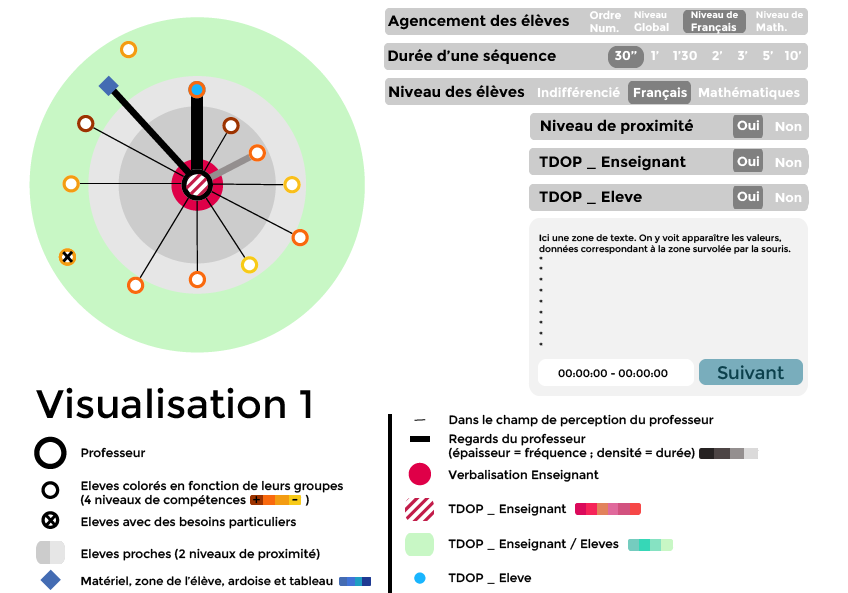
\includegraphics[height=5cm]{visu_cercle.png}
    \end{center}
  \item On pourrait aussi, avec une visualisation du dessus, tracer la trajectoire du regard de l'enseignant, et calculer si il se concentre en moyenne plus sur les élèves du premier rang, ou si il est plus équitablement distriué dans l'espace de la classe. Plus bas une idée de ce type de représentation telle que concue initialement par l'équipe de recherche. Cela étant dit, le problème qui risque de se poser est qu'on ne possède pas de données sur la position de l'enseignant lui même. Peut être pourrait on les entrer à nouveau en se basant sur les vidéos enregistrées ? Ce serait en tout cas un travail long et fastidieux (4h d'enregistrement * une entrée toutes les 500ms = environ 28000 entrées).\\
  \item Enfin, il serait également intéressant de mettre en comparaison les résultats des enseignants novices et expérimentés. Tout d'abord, cela permettrait de comparer à nouveau les coefficients Gini des enseignants (ce qui est fait dans l'article~\cite{SuperViseur} mais pas dans les visualisations en ligne). De plus, étudier les différences de rétroactions permettrait également de mettre en évidence des motifs comportementaux présents uniquements chez les enseignants experts (provenants de leur expérience) qui seraient d'une grande utilité pour la formation de futurs enseignants.
    \begin{center}
      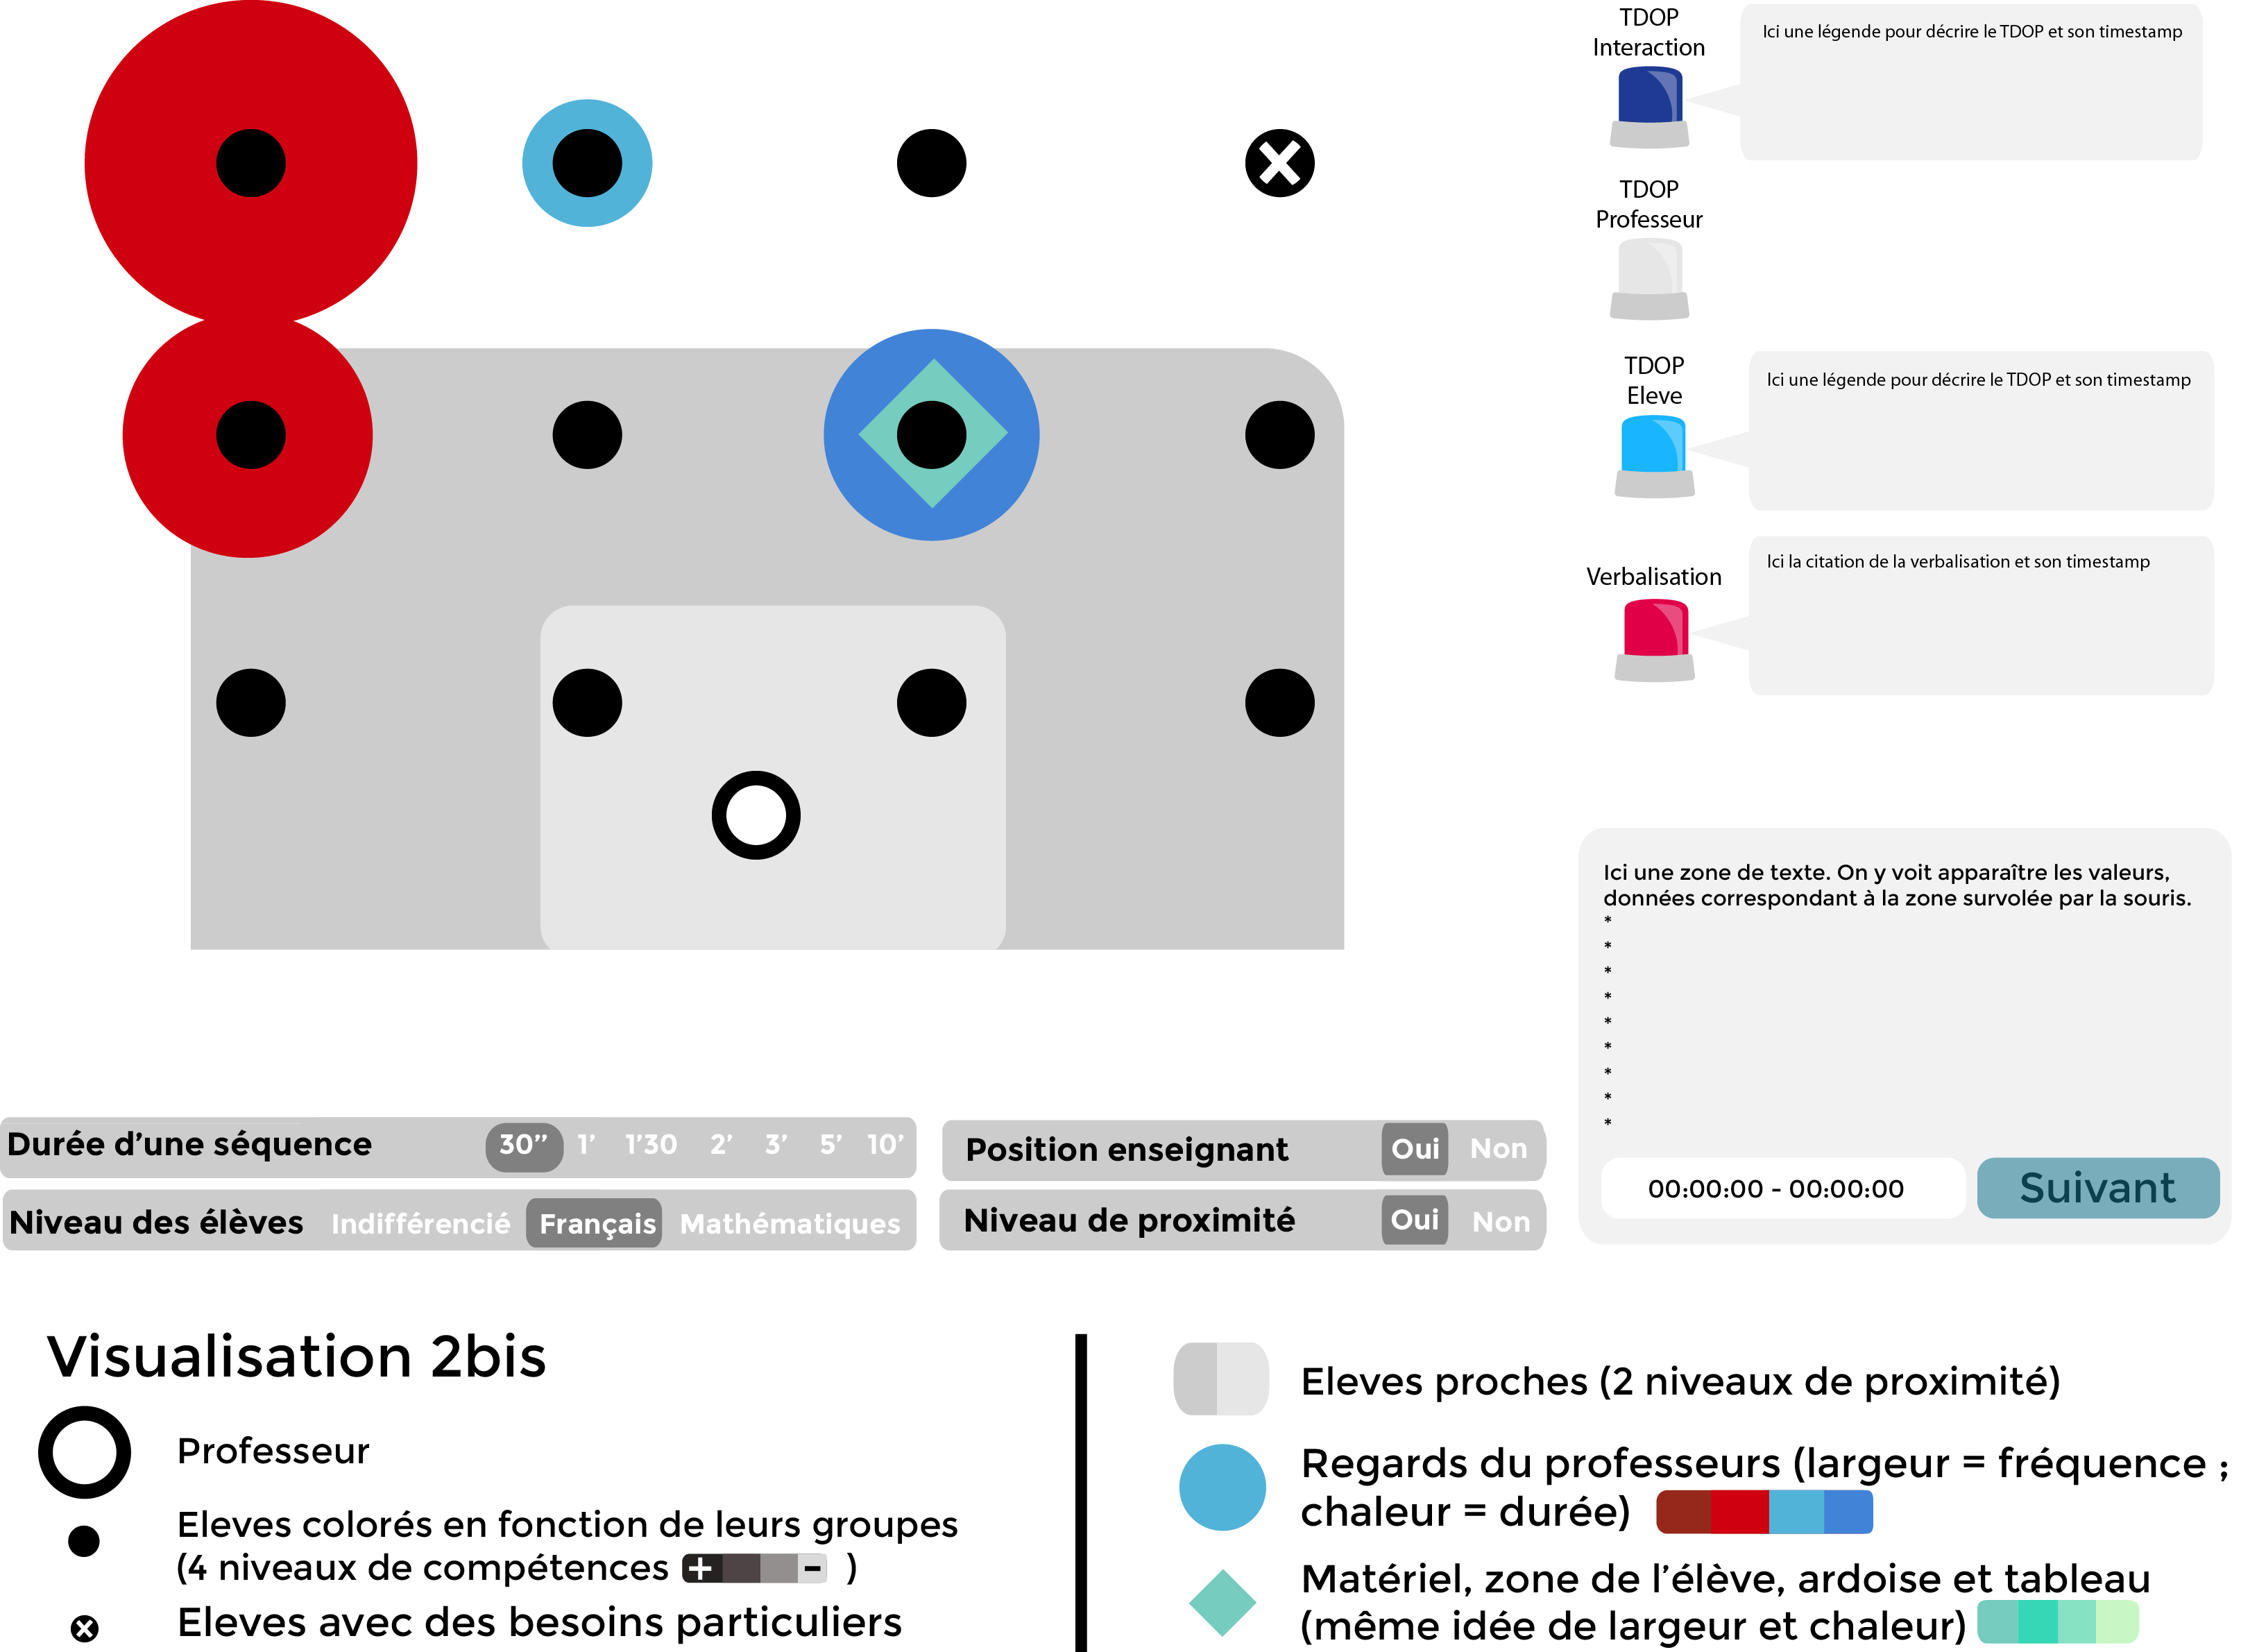
\includegraphics[height=5cm]{visu_dessus.png}
    \end{center}
\end{itemize}

\subsection{Technologies impliquées}
Afin de rendre les visualisations facilement visibles pour d'autres chercheurs (sans avoir nécessairement à télécharger un logiciel, ou des librairies particulières) il parait logique d'utiliser des technologies du Web. Ces dernières sont devenues, lors de ces dernières années, plus que capable de réaliser les calculs nécessaires pour produires ces visualisations en temps réelles. On pourra donc simplement réunir les visualisations sur un site Web dédié (comme c'est déjà le cas pour les visualisations de timeline) et les rendre ainsi instantanément accessibles.\\
Les technologies du Web employées seront donc sans doute l'habituel triplet HTML5+CSS3+Javascript. Afin de pouvoir facilement tracer des graphes, on pourra utiliser la librairie Chart.js. Seulement, certaines des visualisations risquent de ne pas rentrer dans les catégories prédéfinies de Chart.js. Afin de pouvoir les représenter et les animer, on pourra par exemple utiliser la bibliothèque p5.js, permettant de dessiner aisément dans des canvas HTML5.\\

\bibliography{bibliographie}{}
\bibliographystyle{plain}
\end{document}
